
\item Sand is pouring from a pipe at the rate of $ 15 cm^3/minute$. The falling sand forms a cone on the ground such that the height of the cone is always one- third of the radius of the base. How fast is the height of the sand cone increasing at the instant when the height is $4cm$	 


\item A rectangular visiting card is to contain $24 sq.cm.$ of printed matter. The margins at the top and bottom of the card are to be $1 cm$ and the margins on the left and right are to be cm as shown below:

%\newpage
\begin{figure}[h!]
\centering
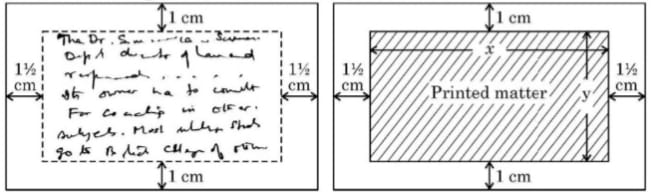
\includegraphics[width=0.8\textwidth]{figs/fig2.jpg}
\label{fig:image2}
\end{figure}

On the basis of the above information, answer the following questions:
\begin{enumerate}
	\item[(i)] Write the expression for the area of the visiting card in terms of x.

	\item[(ii)] Obtain the dimensions of the card of minimum area.



\end{enumerate}



 \item The angle which the line $\frac{x}{1} = \frac{y}{-1} = \frac{z}{2}$ makes with the positive direction of the $y$-axis is:
    \begin{enumerate}[label=(\alph*)]
        \item $\frac{5\pi}{6}$
        \item $\frac{3\pi}{4}$
        \item $\frac{5\pi}{4}$
        \item $\frac{7\pi}{4}$
    \end{enumerate}
    \item Given a curve $y = 7x - x^3$ and $x$ increases at the rate of 2 units per second, the rate at which the slope of the curve is changing when $x = 5$ is:
    \begin{enumerate}[label=(\alph*)]
        \item $-60$ units/sec
        \item $60$ units/sec
        \item $-70$ units/sec
        \item $-140$ units/sec
    \end{enumerate}
     \item The area bounded by the curve $y = \sqrt{x}$, the $y$-axis, and between the lines $y = 0$ and $y = 3$ is:
    \begin{enumerate}[label=(\alph*)]
        \item $2\sqrt{3}$
        \item $27$
        \item $9$
        \item $3$
    \end{enumerate}



\item  Given a curve $ y =7x-x^3 $ and $x$ increases at the rate of 2 units per second.The rate  at which the slope of the curve  is changing,when $x=5$ is:

\begin{enumerate}
\item$-60$ units/sec
\item$60$ units/sec
\item$-70$ units/sec
\item$-140$ units/sec

\end{enumerate}


\item The area of the region bounded by the curve $y^2=4x$ and $x=1$ is:
\begin{enumerate}                                 
\item $\frac{4}{3}$    
\item $\frac{8}{3}$                                                    
 \item $\frac{64}{3}$                                                    
\item $\frac{32}{3}$                                                     
\end{enumerate}                                                       

\item The angle which the line $\frac{x}{1}$=$\frac{y}{-1}$=$\frac{z}{0}$ makes with the positive direction of  Y-axis is:                        
\begin{enumerate}                                     
\item $\frac{5\pi}{6}$  
\item $\frac{3\pi}{4}$              
\item $\frac{5\pi}{4}$                                    
\item $\frac{7\pi}{4}$                                           

\end{enumerate}


\item Area of the region bounded by curve $y^2 = 4x$ and the $X-axis$ between $x = 0$ and $x = 1$ is :
	\begin{enumerate}[label=(\Alph*)]
\item $\frac{2}{3}$
\item $\frac{8}{3}$
\item $3$
\item $\frac{4}{3}$
\end{enumerate}
		\item Given a curve $y = 7x - x^3$ and $x$ increases at the rate of $2 units per second$. The rate at which the slope of the curve is changing, when $x = 5$ is :
		\begin{enumerate}[label=(\Alph*)]
		\item $-60 units/sec$
		\item $60 units/sec$
		\item $-70 units/sec$
		\item $-140 units/sec$
		\end{enumerate}


\end{enumerate}
